\documentclass[letterpaper,10pt, twocolumn]{article}
\usepackage{indentfirst}
\usepackage{listings}
\usepackage{graphicx}
\graphicspath{ {images/} }


\lstset{basicstyle=\ttfamily,
  mathescape=true,
  escapeinside=||}

\begin{document}

\title{\vspace{-2.5cm} \textbf{Face-CNN} \\ \normalsize CS280 Final Project, Spring 2015}
\author{Michelle Nguyen, Allen Tang 22900725}
\date{}

\maketitle

\section{Overview}
	Human attraction based on physical characteristics translates to a picky phenomenon. Individuals value a wide range varying features, preferring certain facial shapes, hair colors, eye colors, hair lengths, etc. We are meeting more people, more quickly than ever, due to advances in social technology. Filtering out potential matches for physical compatibility can be relatively time-consuming.
	
	To solve this problem, we propose a robust feature classifier based on the CNN network by LeCun et al \cite{LeCun}. We will train and test images from a dataset and also from images available on the internet.

\section{Dataset}
We will train our CNN with images and labels taken from the FaceTracer dataset\cite{FaceTracer}. Testing will be done on a held-out part of the dataset and images from internet. The recent increase in personal photos uploaded via social media, on apps (Instagram, Tinder) and websites (Facebook, Match.com) creates a vast dataset suitable and ripe for labeling and testing.


\section{Face Detection}
	Good face detection algorithms have been around for a number of years. The Viola–--Jones algorithm provides relatively quick feature computation, efficient feature selection, and scale and location invariance, suitable for detection of faces on a large dataset.  We will then process faces by by creating a bounding box that will include the subject's headshot. We will implement face detection using OpenCV.

\section{Feature Classification}
	Once we have the faces and bounding box, we will use scale the faces to a fixed image size and then feed the labels into a layered CNN trained on a list of labels. These labels will include such features as gender, race, age, hair\textunderscore color, eye\textunderscore wear, mustache, expression. We will then test the accuracy of our classifier on a held-out set from the FaceTracer database and self-labeled images on the internet. We will train our CNN using Caffe.

\begin{figure}
  \centering
    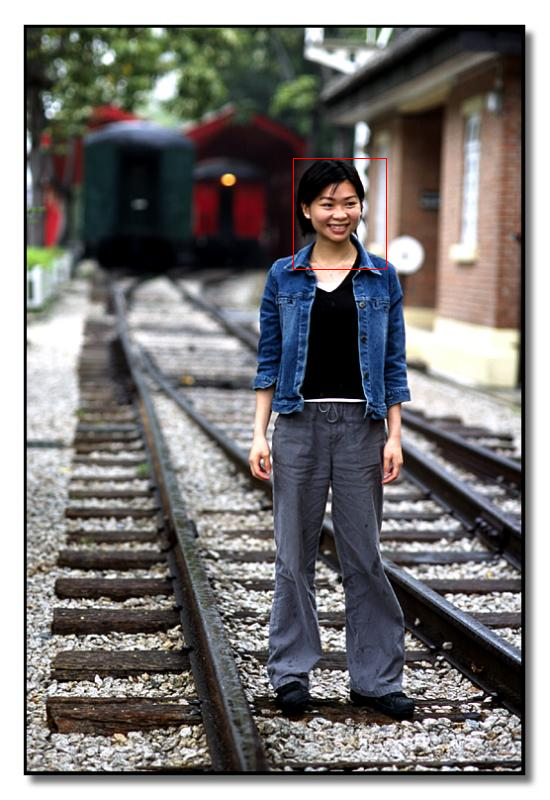
\includegraphics[scale=0.3]{intro-graphics/facerect}
  \caption{Facebox of Woman \cite{FaceTracer}}
  \label{fig:facebox}
\end{figure}







\begin{thebibliography}{9}
\bibitem{FaceTracer}
	"FaceTracer: A Search Engine for Large Collections of Images with Faces," 
	N. Kumar, P. N. Belhumeur, and S. K. Nayar, 
	European Conference on Computer Vision (ECCV), 
	pp.340-353, Oct, 2008.
\bibitem{LeCun}
	P. Sermanet, K. Kavukcuoglu, S. Chintala, and Y. LeCun. Pedestrian
	detection with unsupervised multi-stage feature learning. In CVPR,
	2013.


\end{thebibliography}
\end{document}
